
%%%%%%%%%%%%%%%%%%%%%%%%%%%%%%%%%%%%%%%%%%%%%%%%%%%%%%%%%%{
%\documentclass[twoside,11pt]{article}
\documentclass[UTF8]{ctexart}
%%%%% PACKAGES %%%%%%
\usepackage{pgm2016}
\usepackage{amsmath}
\usepackage{algorithm}
\usepackage[noend]{algpseudocode}
\usepackage{subcaption}
\usepackage[english]{babel}	
\usepackage{paralist}	
\usepackage[lowtilde]{url}
\usepackage{fixltx2e}
\usepackage{listings}
\usepackage{color}
\usepackage{hyperref}
\usepackage{mdframed}

%\usepackage{auto-pst-pdf}
\usepackage{pst-all}
\usepackage{pstricks-add}

%%%%% MACROS %%%%%%
\algrenewcommand\Return{\State \algorithmicreturn{} }
\algnewcommand{\LineComment}[1]{\State \(\triangleright\) #1}
\renewcommand{\thesubfigure}{\roman{subfigure}}
\definecolor{codegreen}{rgb}{0,0.6,0}
\definecolor{codegray}{rgb}{0.5,0.5,0.5}
\definecolor{codepurple}{rgb}{0.58,0,0.82}
\definecolor{backcolour}{rgb}{0.95,0.95,0.92}
\lstdefinestyle{mystyle}{
	backgroundcolor=\color{backcolour},  
	commentstyle=\color{codegreen},
	keywordstyle=\color{magenta},
	numberstyle=\tiny\color{codegray},
	stringstyle=\color{codepurple},
	basicstyle=\footnotesize,
	breakatwhitespace=false,        
	breaklines=true,                
	captionpos=b,                    
	keepspaces=true,                
	numbers=left,                    
	numbersep=5pt,                  
	showspaces=false,                
	showstringspaces=false,
	showtabs=false,                  
	tabsize=2
}
\lstset{style=mystyle}

\newenvironment{problem}[2][问题]
{\begin{mdframed}[backgroundcolor=gray!20] \textbf{#1 #2} \\}
	{\end{mdframed}}

\newenvironment{dingyi}[2][定义]
{\begin{mdframed}[backgroundcolor=gray!20] \textbf{#1 #2} \\}
	{\end{mdframed}}

\newenvironment{dingli}[2][定理]
{\begin{mdframed}[backgroundcolor=gray!20] \textbf{#1 #2} \\}
	{\end{mdframed}}

%%%%%%%%%%%%%%%%%%%%%%%%%%%%%%%%%%%%%%%%%%%%%%%%%%%%%%%%%% 


%%%%%%%%%%%%%%%%%%%%Information%%%%%%%%%%%%%%%%%%%%%%%%%%%
\newcommand\course{sd03431280}
\newcommand\courseName{数值计算方法}
\newcommand\semester{2020·春季}
\newcommand\assignmentNumber{3}
\newcommand\studentName{陈路}
\newcommand\studentEmail{chenlu.scien@gmail.com}
\newcommand\studentNumber{201800301206}
\newcommand\addr{泰山学堂2018级计算机取向}
%%%%%%%%%%%%%%%%%%%%%%%%%%%%%%%%%%%%%%%%%%%%%%%%%%%%%%%%%%



%%%%%%%%%%%%%%%%%%%%%%%%%%%%%%%%%%%%%%%%%%%%%%%%%%%%%%%%%%
    \ShortHeadings{山东大学\quad \semester\quad  \course\quad \courseName}{\addr \quad \studentName \quad \studentNumber}
    \firstpageno{1}
    
    \begin{document}
    
    \title{第\assignmentNumber 章\quad 插值与多项式逼近}
    
    \author{\name \studentName \email \studentEmail \\
    \studentNumber
    }
    
    \maketitle
%%%%%%%%%%%%%%%%%%%%%%%%%%%%%%%%%%%%%%%%%%%%%%%%%%%%%%%%%%
本文首先简要总结插值与多项式逼近的相关知识,包括插值的基本概念和两种常见的插值方法及其误差估计。进而对不同边界条件的样条函数插值进行推导和代码实现,并在实际问题中进行比较。

\section{插值与多项式逼近知识总结}
\subsection{基本概念}
\subsubsection{插值}
给定一系列离散的监测数据点$\left(x_{0}, f\left(x_{0}\right)\right),\left(x_{1}, f\left(x_{1}\right)\right), \cdots,\left(x_{n}, f\left(x_{n}\right)\right)$,假设这些数据都是正确的(没有监测误差),怎样求解非监测点$\left(x \neq x_{i}, i=0,1,2, \cdots, n\right)$的函数值$f(x)$?
这类问题可以被看作是寻找一个函数$f(x)$对给定数据进行拟合,这一过程称为插值.
简单来说,插值就是利用邻近点上已知函数值的加权平均来估计未知函数值.

\subsubsection{多项式逼近}
将实数集映射到自身的最有用且最有名的函数类之一是代数多项式类,即形如下式的函数集合:
\begin{align}
	P_{n}(x)=a_{n} x^{n}+a_{n-1} x^{n-1}+\cdots+a_{1} x+a_{0}\notag
\end{align}
此处$n$是非负整数$a_{0},\cdots,a_{n}$是实常数.
任给一个在有界闭区间上有定义且连续的函数,存在一个多项式可以和给定的函数“接近”到期望的程度。这个结果精确地表示为下面的定理
\begin{dingli}{1}
	设$f$在$[a,b]$上有定义且连续,则对每一个$\varepsilon>0$,存在一个多项式$P(x)$使得对$[a,b]$内的所有$x$均有$|f(x)-P(x)|<\varepsilon$.
\end{dingli}

\subsection{插值方法}
\subsubsection{泰勒多项式逼近}
\begin{dingli}{2}
	设$f \in C^{N+1}[a, b]$,而$x_{0} \in [a,b]$是固定值. 如果$x \in [a,b]$,则有:
	\begin{align}
		f(x)=P_{N}(x)+E_{N}(x)\notag
	\end{align}
	其中$P_{N}(x)$为用来近似$f(x)$的多项式:
	\begin{align}
		f(x) \approx P_{N}(x)=\sum_{k=0}^{N} \frac{f^{(k)}\left(x_{0}\right)}{k !}\left(x-x_{0}\right)^{k}\notag
	\end{align}
	误差项$E_{N}(x)$形如:
	\begin{align}
		E_{N}(x)=\frac{f^{(N+1)}(c)}{(N+1) !}\left(x-x_{0}\right)^{N+1}\notag
	\end{align}
	其中$c$为$x$和$x_{0}$之间的某个值$c=c(x)$.
\end{dingli}
泰勒多项式的精度随着$N$的增长而提高,通常,任何给定多项式的精度都将随着$x$远离中心点$x_{0}$而降低,因此必须选择足够大的$N$,并限制$|x-x_{0}|$的最大值,才能使误差不超过给定限度.
假设选择区间宽度为$2R$,而$x_{0}$位于区间中心(即$|x-x_{0}|<R$),则误差绝对值满足关系:
\begin{align}
	\text { |误差| }=\left|E_{N}(x)\right| \leqslant \frac{M R^{N+1}}{(N+1) !}\notag
\end{align}
其中,$M \geqslant \max \left\{\left|f^{N+1}(z)\right|: x_{0}-R \leqslant z \leqslant x_{0}+R\right\}$

\subsubsection{拉格朗日插值多项式逼近}
$n$次拉格朗日插值多项式的定义
\begin{dingyi}{1}
	如果$x_{0},x_{1},\cdots,x_{N}$是$N+1$个不同的点且函数$f$在这些点处的函数值已知,则存在一个次数最高为$N$的多项式$P_{N}(x)$,具有以下形式:
	\begin{align}
		P_{N}(x)=f\left(x_{0}\right) L_{N, 0}(x)+\cdots+f\left(x_{N}\right) L_{N, N}(x)=\sum_{k=0}^{N} f(x_{k}) L_{N, k}(x)\notag
	\end{align}
	其中,对每一个$k=0,1,\cdots,N$,$L_{N, k}(x)$定义为
	\begin{align}
		L_{N, k}(x)=\frac{\left(x-x_{0}\right)\left(x-x_{1}\right) \cdots\left(x-x_{k-1}\right)\left(x-x_{k+1}\right) \cdots\left(x-x_{N}\right)}{\left(x_{k}-x_{0}\right)\left(x_{k}-x_{1}\right) \cdots\left(x_{k}-x_{k-1}\right)\left(x_{k}-x_{k+1}\right) \cdots\left(x_{k}-x_{N}\right)}\notag
	\end{align}
	(注意$\left(x-x_{k}\right)$和$\left(x_{k}-x_{k}\right)$不出现在上式右端)引入累乘表示法
	\begin{align}
		L_{N, k}(x)=\frac{\prod_{j=0 \atop j \neq k}^{N}\left(x-x_{j}\right)}{\prod_{j=0 \atop j \neq k}^{N}\left(x_{k}-x_{j}\right)}\notag
	\end{align}
\end{dingyi}
拉格朗日插值多项式逼近
\begin{dingli}{1}
	设$f \in C^{N+1}[a,b]$,且$x_{0},x_{1},\cdots,x_{N} \in [a,b]$为$N+1$个节点. 如果$x \in [a,b]$,则
	\begin{align}
		f(x)=P_{N}(x)+E_{N}(x)\notag
	\end{align}
	其中$P_{N}(x)$为用来近似$f(x)$的多项式:
	\begin{align}
		f(x) \approx P_{N}(x)=\sum_{k=0}^{N} f(x_{k}) L_{N, k}(x)\notag
	\end{align}
	误差项$E_{N}(x)$形如:
	\begin{align}
		E_{N}(x)=\frac{\left(x-x_{0}\right)\left(x-x_{1}\right) \cdots\left(x-x_{N}\right) f^{(N+1)}(c)}{(N+1) !}\notag
	\end{align}
	其中$c$为区间$[a,b]$的某个值$c=c(x)$.
\end{dingli}

\section{分析讨论题}


\begin{problem}{1}
基于不同边界条件的样条函数计算公式推导
\begin{enumerate}
	\item 自然边界
	\item 固定边界
	\item 周期边界
	\item 强制第一个子区间和第二个子区间样条多项式的三阶导数相等,倒数第二个子区间和最后一个子区间的三次样条函数的三阶导数相等
\end{enumerate}
\end{problem}
\textbf{解}:\\
\begin{dingyi}{1}
	 假设$\{(x_k,y_k)\}_{k=0}^{N}$有N+1个点,其中$a=x_0<x_1<\cdots <x_N=b$。如果存在N个三次多项式$S_k(x)$,系数为$s_{k,0},s_{k,1},s_{k,2},s_{k,3}$,满足如下性质:
	\begin{enumerate}
		\item I. $S(x)=S_k(x)=s_{k,0}+s_{k,1}(x-x_k)+s_{k,2}(x-x_k)^2+s_{k,3}(x-x_k)^3,x\in [x_k,x_{k+1}],\quad k=0,1,2,\cdots,N-1$
		\item II. $S(x_k)=y_k,\quad k=0,1,\cdots ,N$
		\item III. $S_k(x_{k+1})=S_{k+1}(x_{k+1}),\quad k=0,1,\cdots ,N-2$
		\item IV. $S_k^{'}(x_{k+1})=S_{k+1}^{'}(x_{k+1}),\quad k=0,1,\cdots ,N-2$
		\item V. $S_k^{''}(x_{k+1})=S_{k+1}^{''}(x_{k+1}),\quad k=0,1,\cdots ,N-2$
	\end{enumerate}
	则称函数$S_(x)$为三次样条函数.
\end{dingyi}
因为$S^{''}(x)$在区间$[x_0,x_N]$内是分段线性的,根据拉格朗日插值有:
\begin{align}
	S_k^{''}(x)=S^{''}(x_k)\frac{x-x_{k+1}}{x_k-x_{k+1}}+S^{''}(x_{k+1})\frac{x-x_k}{x_{k+1}-x_k} \notag
\end{align}
令$m_k=S^{''}(x_k),m_{k+1}=S^{''}(x_{k+1})$和$h_k=x_{k+1}-x_k$得:
\begin{align}
	S_k^{''}(x)=\frac{m_k}{h_k}(x_{k+1}-x)+\frac{m_{k+1}}{h_k}(x-x_k)\label{eq:1}
\end{align}
对上式\ref{eq:1}积分两次可得
\begin{align}
	S_k(x)=\frac{m_k}{6h_k}(x_{k+1}-x)^3+\frac{m_{k+1}}{6h_k}(x-x_k)^3+p_k(x_{k+1}-x)+q_k(x-x_k)\label{eq:2}
\end{align}
将$x_k,x_{k+1}$代入上式\ref{eq:2}中,且有$y_k=S_k(x_k),y_{k+1}=S_k(x_{k+1})$,可得:
\begin{align}
	y_k=\frac{m_k}{6}h_k^2+p_k h_k , y_{k+1}=\frac{m_{k+1}}{6}h_k^2+q_k h_k  \notag
\end{align}
解出$p_k,q_k$代入\ref{eq:1}式中可得:
\begin{align}
	S_k(x)=\frac{m_k}{6h_k}(x_{k+1}-x)^3+\frac{m_{k+1}}{6h_k}(x-x_k)^3+(\frac{y_k}{h_k}-\frac{m_k h_k}{6})(x_{k+1}-x)+(\frac{y_{k+1}}{h_k}-\frac{m_{k+1}h_k}{6})(x-x_k) \notag
\end{align}
求导可得:
\begin{align}
	S_k^{'}(x)=-\frac{m_k}{2h_k}(x_{k+1}-x)^2+\frac{m_{k+1}}{2h_k}(x-x_k)^2-(\frac{y_k}{h_k}-\frac{m_k h_k}{6})+(\frac{y_{k+1}}{h_k}-\frac{m_{k+1}h_k}{6}) \label{eq:3}
\end{align}
将$x_k,x_{k-1}$分别代入上式\ref{eq:3}可得:
\begin{align}
	S_k^{'}(x_k)=-\frac{m_k}{3}h_k-\frac{m_{k+1}}{6}h_k+d_k \label{eq:4}\\
	S_k^{'}(x_{k-1})=\frac{m_k}{3}h_{k-1}+\frac{m_{k-1}}{6}h_{k-1}+d_{k-1} \label{eq:5}
\end{align}
由性质IV和上式\ref{eq:4}\ref{eq:5}得:
\begin{align}
	h_{k-1}m_{k-1}+2(h_{k-1}+h_k)m_k+h_km_{k+1}=u_k \label{eq:*}\\
	u_k=6(d_k-d_{k-1}),d_k=\frac{y_{k+1}-y_k}{h_k},h_k=x_{k+1}-x_k \notag
\end{align}
由于式\ref{eq:*}中的未知数为$\{m_k\}$,而其他项可由数据点集$\{(x_k,y_k)\}$进行数学计算得到.
而方程\ref{eq:*}中包含N+1个未知数,具有N-1个线性方程,因而需要另外两个方程.所以需要对两端点$x_0,x_N$的微分加一些限制.\\

\textbf{1. 自然边界}\\
自然边界条件为:$S^{''}(a)=0,S^{''}(b)=0$\\
则求解的方程组为:
\begin{equation}
	\begin{cases}
		2(h_0+h_1)m_1+h_1m_2=u_1 \\
		h_{k-1}m_{k-1}+2(h_{k-1}+h_k)m_k+h_km_{k+1}=u_k,\quad k=2,3,\cdots ,N-2 \\
		h_{N-2}m_{N-2}+2(h_{N-2}+h_{N-1})m_{N-1}=u_{N-1} \notag
	\end{cases}
\end{equation}
可转化为矩阵运算:
\begin{equation}
	\left(
	\begin{array}{ccccc}
		1 & 0 & 0 & \cdots & 0 \\
		h_0 & 2(h_0+h_1) & h_1 & 0 & \vdots\\
		0 & h_1 & 2(h_1+h_2) & h_2 & \vdots\\
		\vdots & \ddots & \ddots & \ddots & 0\\
		0 & \cdots & h_{N-2} & 2(h_{N-2}+h_{N-1}) & h_{N-1}\\
		0 & \cdots & 0 & 0 & 1 
	\end{array}
	\right)
	\left(
	\begin{array}{c}
		m_0\\
		m_1\\
		m_2\\
		m_3\\
		\vdots \\
		m_N
	\end{array}
	\right)
	=
	\left(
	\begin{array}{c}
		0\\
		u_1\\
		u_2\\
		\vdots \\
		u_{N-1}\\
		0
	\end{array}
	\right) \notag
\end{equation}
代码实现如下:
\begin{lstlisting}[language=matlab]
function S1 = naturalfuc(X,Y)
N=length(X)-1;
H=diff(X);
D=diff(Y)./H;
A=H(2:N-1);
B=2*(H(1:N-1)+H(2:N));
C=H(2:N);
U=6*diff(D);
B(1)=B(1)-H(1)/2;
B(N-1)=B(N-1)-H(N)/2;

for k=2:N-1
	temp=A(k-1)/B(k-1);
	B(k)=B(k)-temp*C(k-1);
	U(k)=U(k)-temp*U(k-1);
end
M(N)=U(N-1)/B(N-1);
for k=N-2:-1:1
	M(k+1)=(U(k)-C(k)*M(k+2))/B(k);
end
M(1)=0;
M(N+1)=0;
for k=0:N-1
	S1(k+1,1)=(M(k+2)-M(k+1))/(6*H(k+1));
	S1(k+1,2)=M(k+1)/2;
	S1(k+1,3)=D(k+1)-H(k+1)*(2*M(k+1)+M(k+2))/6;
	S1(k+1,4)=Y(k+1);
end
end
\end{lstlisting}

\textbf{2. 固定边界:}\\
只需对式\ref{eq:*}的方程$1$到方程$N-1$进行重写,得到一个包含$m_1,m_2,\cdots ,m_{N-1}$的三角线性方程组$HM=V$,即:
\begin{equation}
	\left(
	\begin{array}{ccccc}
		b_{1} & c_{1} & 0 & \cdots & 0 \\
		a_{1} & b_{2} & c_{2} & \cdots & 0\\
		\vdots & \ddots & \ddots & \ddots & \vdots \\
		0 & \cdots & a_{N-3} & b_{N-2} & c_{N-2} \\
		0 & \cdots & 0 & a_{N-2} & b_{N-1} 
	\end{array}
	\right)
	\left(
	\begin{array}{c}
		m_0\\
		m_1\\
		m_2\\
		\vdots \\
		m_{N-2}\\
		m_{N-1}
	\end{array}
	\right)
	=
	\left(
	\begin{array}{c}
		v_1\\
		v_2\\
		\vdots \\
		v_{N-2}\\
		v_{N-1}
	\end{array}
	\right)\notag
\end{equation}
代码实现如下:
\begin{lstlisting}[language=matlab]
function S4 = epfuc(X,Y)
N=length(X)-1;
H=diff(X);
D=diff(Y)./H;
A=H(2:N-1);
B=2*(H(1:N-1)+H(2:N));
C=H(2:N);
U=6*diff(D);

B(1)=B(1)-H(1)/2;
U(1)=U(1);
B(N-1)=B(N-1)-H(N)/2;
U(N-1)=U(N-1);
for k=2:N-1
	temp=A(k-1)/B(k-1);
	B(k)=B(k)-temp*C(k-1);
	U(k)=U(k)-temp*U(k-1);
end
M(N)=U(N-1)/B(N-1);
for k=N-2:-1:1
	M(k+1)=(U(k)-C(k)*M(k+2))/B(k);
end
M(1)=1;
M(N+1)=-1;
for k=0:N-1
	S4(k+1,1)=(M(k+2)-M(k+1))/(6*H(k+1));
	S4(k+1,2)=M(k+1)/2;
	S4(k+1,3)=D(k+1)-H(k+1)*(2*M(k+1)+M(k+2))/6;
	S4(k+1,4)=Y(k+1);
end
end
\end{lstlisting}

\textbf{3. 周期边界}\\
周期边界条件为:$S_0^{'}(x_0)=S_N^{'}(x_n),\qquad S_0^{''}(x_0)=S_N^{''}(x_n)$\\
带入式\ref{eq:*}可得到方程组:
\begin{equation}
	\begin{cases}
		2h_0+2h_1-\frac{h_0^2}{2(h_0+h_1)})m_1+h_1m_2-\frac{h_{N-1}h_0}{2(h_0+h_1)}m_{N-1}=u_1-\frac{3h_0(d_0-d_{N-1})}{(h_0+h_1)} \\
		h_{k-1}m_{l-1}+2(h_{k1}+h_k)m_k+h_km_{k+1}=u_k,\quad k=2,3,\cdots,N-2 \\
		-\frac{h_{N-1}h_0}{2(h_0+h_1)}m_1+h_{N-2}m_{N-2}+2(h_{N-2}+2h_{N-1})m_{N-1}-\frac{h_{N-1}^2}{2(h_0+h_1)}m_{N-1}=u_{N-1}-h_{N-1}\frac{3(d_0-d_{N-1})}{(h_0+h_1)} \notag
	\end{cases}
\end{equation}
可转化为矩阵运算:
\begin{equation}
	\left(
	\begin{array}{ccccc}
		1 & 0 & 0 & \cdots & 0 \\
		h_0 & 2(h_0+h_1) & h_1 & 0 & \vdots\\
		0 & h_1 & 2(h_1+h_2) & h_2 & \vdots\\
		\vdots & \ddots & \ddots & \ddots & 0\\
		0 & \cdots & h_{N-2} & 2(h_{N-2}+h_{N-1}) & h_{N-1}\\
		h_0+h_{N-1} & h_0 & \cdots & h_{N-1} & h_{N}+h_{N-1} 
	\end{array}
	\right)
	\left(
	\begin{array}{c}
		m_0\\
		m_1\\
		m_2\\
		m_3\\
		\vdots \\
		m_{N}
	\end{array}
	\right)
	=
	\left(
	\begin{array}{c}
		0\\
		u_1\\
		u_2\\
		\vdots \\
		u_{N-1}\\
		\frac{3(d_0-d_{N-1})}{(h_0+h_1)}
	\end{array}
	\right)
\end{equation}
代码实现如下:
\begin{lstlisting}[language=matlab]
function S5 = sicfuc(X,Y)
N=length(X)-1;
H=diff(X);
D=diff(Y)./H;
A=H(2:N-1);
B=2*(H(1:N-1)+H(2:N));
C=H(2:N);
U=6*diff(D);
B(1)=B(1)-H(1)/2;
B(N-1)=B(N-1)-H(N)/2;

for k=2:N-1
	temp=A(k-1)/B(k-1);
	B(k)=B(k)-temp*C(k-1);
	U(k)=U(k)-temp*U(k-1);
end
M(N)=U(N-1)/B(N-1);
for k=N-2:-1:1
	M(k+1)=3((U(k)-C(k)*M(k+2))/B(k));
end
M(1)=0;
M(N+1)=3(D(0)-D(N-1))/(H(0)+H(1));
for k=0:N-1
	S1(k+1,1)=(M(k+2)-M(k+1))/(6*H(k+1));
	S1(k+1,2)=M(k+1)/2;
	S1(k+1,3)=D(k+1)-H(k+1)*(2*M(k+1)+M(k+2))/6;
	S1(k+1,4)=Y(k+1);
end
end
\end{lstlisting}

\textbf{4. 特定边界}\\
边界条件为:
\begin{align}
	S_0^{'''}(x_1)=S_1^{'''}(x_1),\qquad S_{N-2}^{'''}(x_{N-1})=S_{N-1}^{'''}(x_{N-1})\notag
\end{align}
可得到如下矩阵方程:\\
\begin{equation}
\left(
\begin{array}{ccccc}
h_1 & -(h_0+h_1) & h_0 & \cdots & 0 \\
h_0 & 2(h_0+h_1) & h_1 & 0 & \vdots\\
0 & h_1 & 2(h_1+h_2) & h_2 & \vdots\\
\vdots & \ddots & \ddots & \ddots & 0\\
0 & \cdots & h_{N-2} & 2(h_{N-2}+h_{N-1}) & h_{N-1}\\
0  & \cdots & h_{N-1} &-(h_{N-2}+h_{N-1}) & h_{N-2}
\end{array}
\right)
\left(
\begin{array}{c}
m_0\\
m_1\\
m_2\\
m_3\\
\vdots \\
m_{N-1}\\
m_{N}
\end{array}
\right)
=
\left(
\begin{array}{c}
0\\
u_1\\
u_2\\
\vdots \\
u_{N-1}\\
0
\end{array}
\right)\notag
\end{equation}
代码实现如下:
\begin{lstlisting}[language=matlab]
function S6 = 3CIfuc(X,Y)
N=length(X)-1;
H=diff(X);
D=diff(Y)./H;
A=H(2:N-1);
B=2*(H(1:N-1)+H(2:N));
C=H(2:N);
U=6*diff(D);

B(1)=B(1)-H(1)/2;
U(1)=U(1);
B(N-1)=B(N-1)-H(N)/2;
U(N-1)=U(N-1);
for k=2:N-1
	temp=A(k-1)/B(k-1);
	B(k)=B(k)-temp*C(k-1);
	U(k)=U(k)-temp*U(k-1);
end
M(N)=U(N-1)/B(N-1);
for k=N-2:-1:1
	M(k+1)=(U(k)-C(k)*M(k+2))/B(k);
end
M(1)=0;
M(N+1)=0;
for k=0:N-1
	S2(k+1,1)=(M(k+2)-M(k+1))/(6*H(k+1));
	S2(k+1,2)=M(k+1)/2;
	S2(k+1,3)=D(k+1)-H(k+1)*(2*M(k+1)+M(k+2))/6;
	S2(k+1,4)=Y(k+1);
end
end
\end{lstlisting}
按上述四种方法求解方程组可得到$\{m_k\}$序列,计算样条系数:
\begin{align}
	s_{k,0}=y_k, s_{k,1}=d_k-\frac{h_k(2m_k+m_{k+1})}{6}\notag \\
	s_{k,2}=\frac{m_k}{2}, s_{k,3}=\frac{m_{k+1}-m_k}{6h_k}\notag 
\end{align}
每个三次多项式为:
\begin{align}
	S_k(x)=((s_{k,3}(x-x_k)+s_{k,2})(x-x_k)+s_{k,1})(x-x_k)+y_k \notag
\end{align}
带入求解即可.


\begin{problem}{2}
	以$y=sin(x)$为例,在$[0,T]$区间内生成$11$个、$21$个数据点,设计算法或程序,用上述$4$个边界条件,分别计算其样条插值,并作图比较,分析其差异性.
\end{problem}
\textbf{解}:\\
图像如下\ref{fig:graph}:
\begin{figure}[H]
	\begin{center}
		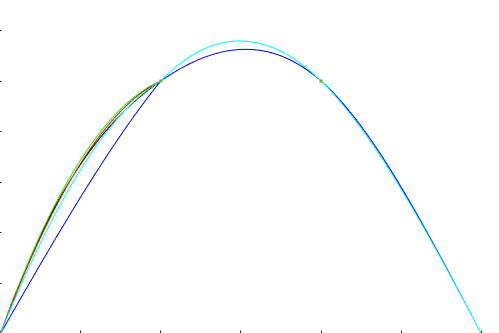
\includegraphics[width=0.7\columnwidth]{figures/graph.png}
		\caption{函数$y=sin(x)$不同样条插值示意图}
		\label{fig:graph}
	\end{center}
\end{figure}
除周期边界外,其他各边界条件拟合良好.\\

\end{document}
